%++++++++++++++++++++++++++++++++++++++++
\documentclass[a4paper,14pt]{extreport}

\usepackage{cmap} % Улучшенный поиск русских слов в полученном pdf-файле
\usepackage[T2A]{fontenc} % Поддержка русских букв
\usepackage[utf8]{inputenc} % Кодировка utf8
\usepackage[english,russian]{babel} % Языки: русский, английский
%\usepackage{pscyr} % Нормальные шрифты

\usepackage{pdfpages}

\usepackage{enumitem}

\usepackage[14pt]{extsizes}

\usepackage{caption}
\captionsetup{labelsep=endash}
\captionsetup[figure]{name={Рисунок}}

\usepackage{amsmath}
\usepackage{geometry}
\geometry{left=30mm}
\geometry{right=10mm}
\geometry{top=20mm}
\geometry{bottom=20mm}



\usepackage{titlesec}
\titleformat{\section}
	{\normalsize\bfseries}
	{\thesection}
	{1em}{}
\titlespacing*{\chapter}{0pt}{-30pt}{8pt}
\titlespacing*{\section}{\parindent}{*4}{*4}
\titlespacing*{\subsection}{\parindent}{*4}{*4}


\usepackage{mathtools}
\usepackage{float}
\DeclarePairedDelimiter\bra{\langle}{\rvert}
\DeclarePairedDelimiter\ket{\lvert}{\rangle}
\DeclarePairedDelimiterX\braket[2]{\langle}{\rangle}{#1 \delimsize\vert #2}

\usepackage{setspace}
\onehalfspacing % Полуторный интервал
\frenchspacing
\usepackage{indentfirst} % Красная строка
\usepackage{titlesec}
\titleformat{\chapter}{\LARGE\bfseries}{\thechapter}{20pt}{\LARGE\bfseries}
\titleformat{\section}{\Large\bfseries}{\thesection}{20pt}{\Large\bfseries}
\usepackage{listings}
\usepackage{xcolor}
\lstdefinestyle{rustlang}{
    language=Rust,
    backgroundcolor=\color{white},
    basicstyle=\footnotesize\ttfamily,
    keywordstyle=\color{purple},\part{title}
    stringstyle=\color{green},
    commentstyle=\color{gray},
    numbers=left,
    stepnumber=1,
    numbersep=5pt,
    frame=single,
    tabsize=4,
    captionpos=t,
    breaklines=true,
    breakatwhitespace=true,
    escapeinside={\#*}{*)},
    morecomment=[l][\color{magenta}]{\#},
    columns=fullflexible
}
\usepackage{pgfplots}
\usetikzlibrary{datavisualization}
\usetikzlibrary{datavisualization.formats.functions}

\usepackage{graphicx}
\newcommand{\img}[3] {
    \begin{figure}[h]
        \center{\includegraphics[height=#1]{img/#2}}
        \caption{#3}
        \label{img:#2}
    \end{figure}
}
\newcommand{\boximg}[3] {
    \begin{figure}[h]
        \center{\fbox{\includegraphics[height=#1]{assets/img/#2}}}
        \caption{#3}
        \label{img:#2}
    \end{figure}
}
\usepackage[justification=centering]{caption} % Настройка подписей float объектов

\usepackage[unicode,pdftex]{hyperref} % Ссылки в pdf
\hypersetup{hidelinks}

\newcommand{\code}[1]{\texttt{#1}}
\usepackage{icomma} % Интеллектуальные запятые для десятичных чисел
\usepackage{csvsimple}

\usepackage{color} %use color
\definecolor{mygreen}{rgb}{0,0.6,0}
\definecolor{mygray}{rgb}{0.5,0.5,0.5}
\definecolor{mymauve}{rgb}{0.58,0,0.82}

%Customize a bit the look
\lstset{ %
	backgroundcolor=\color{white}, % choose the background color; you must add \usepackage{color} or \usepackage{xcolor}
	basicstyle=\footnotesize, % the size of the fonts that are used for the code
	breakatwhitespace=true, % sets if automatic breaks should only happen at whitespace
	breaklines=true, % sets automatic line breaking
	captionpos=t, % sets the caption-position to bottom
	%commentstyle=\color{mygreen}, % comment style
	%deletekeywords={...}, % if you want to delete keywords from the given language
	escapeinside={\%*}{*)}, % if you want to add LaTeX within your code
	%extendedchars=true, % lets you use non-ASCII characters; for 8-bits encodings only, does not work with UTF-8
	frame=single, % adds a frame around the code
	%keepspaces=true, % keeps spaces in text, useful for keeping indentation of code (possibly needs columns=flexible)
	keywordstyle=\color{blue}, % keyword style
	% language=Octave, % the language of the code
	%morekeywords={*,...}, % if you want to add more keywords to the set
	numbers=left, % where to put the line-numbers; possible values are (none, left, right)
	numbersep=5pt, % how far the line-numbers are from the code
	numberstyle=\tiny\color{mygray}, % the style that is used for the line-numbers
	%rulecolor=\color{black}, % if not set, the frame-color may be changed on line-breaks within not-black text (e.g. comments (green here))
	%showspaces=false, % show spaces everywhere adding particular underscores; it overrides 'showstringspaces'
	%showstringspaces=false, % underline spaces within strings only
	%showtabs=false, % show tabs within strings adding particular underscores
	stepnumber=1, % the step between two line-numbers. If it's 1, each line will be numbered
	%stringstyle=\color{mymauve}, % string literal style
	tabsize=2, % sets default tabsize to 2 spaces
	%title=\lstname % show the filename of files included with \lstinputlisting; also try caption instead of title
}

\begin{document}
	
		
\includepdf[pages=-]{include/title.pdf}

		
\includepdf[pages=-]{include/task.pdf}
		
		\setcounter{page}{3}
		\renewcommand{\contentsname}{Содержание} % Переименовать table of contents
		\tableofcontents

		\thispagestyle{empty}
		\chapter*{Введение}
		\addcontentsline{toc}{chapter}{Введение}
		В наше время построение трехмерных изображений является одной из
			множества задач компьютерной графики, но существующие алгоритмы,
			которые дают возможность получить реалистичное изображение, работают
			крайне медленно. Также алгоритмы, которые позволяют построить
			нагруженные сцены в реальном времени, не учитывают все особенности
			объектов изображения и реализуются при помощи графических процессоров.
		\par Целью практики является получение навыков разработки программного 
			обеспечения, реализующего отображение сцены, приобретение опыта 
			самостоятельной разработки программного продукта, изучение средств 
			автоматизации развёртывания, сборки и тестирования программы
		\par Задачи, необходимые к выполнению для достижения данной цели:
		\begin{enumerate} 
        			\item Изучить документацию Gitlab CI/CD, Docker, Qt, Qt Test, Qt Widgets, ffmpeg
        			\item Создать программу, принимающую данные о сцене, содержащей 
				объекты, и создающую изображение. Использовать алгоритм Z-буфера с тенями для отрисовки сцены.
			\item Создать сценарий gitlab-ci.yml автоматизации сборки, тестирования, 
				выполнения замерного эксперимента и получения данных будущего 
				исследования.
			\item Выбрать готовый подходящий для поставленных задач отрисовки образ 
				docker.
			\item Создать три сцены разной сложности (по числу 
				полигонов, из которых они состоят) для демонстрации 
				работоспособности всего конвейера.
			\item Создать модульный тест для демонстрации работоспособности системы.
			\item Создать сценарий исследования зависимости времени выполнения от 
				количества полигонов.
    		\end{enumerate} 
		
		\chapter{Знакомство с документацией}
		Далее представлено краткое изложение изученной документации, 
		необходимой для разработки программного продукта и автоматизации его 
		развёртки. Указаны ссылки на использованные материалы.
		\section{Gitlab CI/CD}
		GitLab CI/CD — это инструмент для разработки программного обеспечения с 		использованием непрерывных методологий. CI (Continuous Integration) — 				непрерывная интеграция. Каждое изменение, 
		представленное в приложении, даже в ветках разработки, фиксируется и 
		тестируется автоматически и непрерывно. CD (Continuous Deployment) —
		непрерывная автоматическая развёртка приложения.
		\par GitLab CI/CD использует ряд концепций для описания и выполнения 
сборки и развертывания [1]:
		\begin{enumerate} 
        			\item Pipeline (сборочная линия) — это компонент верхнего уровня, 
состоящий из: 
		 	\begin{enumerate} 
        				\item Задания (job), которые определяют, что делать. Они могут  присутствовать в любом количестве и иметь ограничения на  выполнение
				\item Стадии (stage), которые определяют, когда выполнять задания. 
    			\end{enumerate} 
			\begin{lstlisting}[label=some-code,caption= пример задачи «Generate image» из стадии «gen\_image»]
			Generate image:
  			stage: gen_image
  			script:
    				- cd new_code
    				- bash gen_image.sh
			\end{lstlisting}
			\par Задания выполняются runner’ами. Несколько заданий на одной 
			стадии выполняются параллельно, если имеется достаточное 
			количество одновременно работающих runner’ов. Если все задания 
			на этапе выполняются успешно, конвейер переходит к следующему 
			этапу. Если какое-либо задание на этапе завершается сбоем, 
			следующий этап (обычно) не выполняется, и конвейер завершается 
			досрочно.
			\par Для задания также можно объявить зависимости:
			\begin{lstlisting}[label=some-code,caption= пример изпользования «needs»]
			needs: 
    				- Unit tests
    				- Func tests
			\end{lstlisting}
			\par В данном примере текущее задание будет выполнено лишь в случае 
			успешного выполнения задания «Unit tests» и «Func tests»
			\item Артефакты
			\par Задания могут оставлять архив файлов и каталогов — артефакт 				задания. Можно загружать артефакты с помощью пользовательского 				интерфейса GitLab. Чтобы создать артефакты заданий, нужно 					использовать ключевое слово «artifacts» в файле .gitlab-ci.yml
			\begin{lstlisting}[label=some-code,caption= пример изпользования «artifacts»]
			  artifacts:
    				paths:
      					- new_code/img.png
    			expire_in: 7 days
			\end{lstlisting}
			\par В примере после выполнения текущего задания к артефактам 					добавятся файлы, соответствующие пути «new\_code/img.png»,
			а время хранения этих артефактов составит 7 дней
			\item gitlab-ci.yml
			Были изучены основные синтаксические конструкции и правила 
			построения .gitlab-ci.yml файла. Были рассмотрены такие ключевые 					слова, как:
			\begin{enumerate} 
        				\item before\_script (команды, выполняемые до основного 						скрипта)
				\item image (клонирование образа docker)
				\item stage (определение стадий сборочной линии)
				\item script (команды основного скрипта)
				\item needs (определение зависимостей и необходимых 						артефактов предыдущих стадий конвейера)
			\end{enumerate} 
				\begin{lstlisting}[label=some-code,caption= пример изпользования ключевых слов в .gitlab-ci.yml]
				Timer:
  					stage: calculate_time
					image: python
					before_script:
						- pip install matplotlib
					script:
						- cd new_code
						- bash gen_time.sh
					artifacts:
 						paths:
							- new_code/graph.png
						expire_in: 7 days
					needs:
						- job: Release build
						artifacts: true
				\end{lstlisting}
				В данном примере описано задание “ Timer” из стадии 						“calculate\_time”, которому необходим docker образ python. Перед 						основным скриптом происходит установка библиотеки 							matplotlib для построения графиков и диаграмм языка Python. 					Основной скрипт запускает Bash скрипт, 
				предварительно переходя в директорию new\_code, оставляя 						артефакты по указанному пути new\_code/graph.png. Это 						задание выполнится только при условии успешного 							выполнения задания Release build и при наличии 								соответствующих этому этапу артефактов.
    		\end{enumerate} 
		\section{Docker}
		Была изучена документация Docker [2] и рассмотрен пример создания 
		Dockerfile.
		\begin{lstlisting}[label=some-code,caption= пример Dockerfile]
			FROM alpine:3.9 as builder

			RUN apk update && apk add ca-certificates tzdata

			FROM scratch

			COPY --from=builder /etc/ssl/certs/ca-certificates.crt /etc/ssl/certs/
			COPY --from=builder /usr/share/zoneinfo /usr/share/zoneinfo/

			COPY main /
			CMD ["/main"]
		\end{lstlisting}
		В данном примере:
		\begin{enumerate}
			\item  FROM задаёт базовый (родительский) образ, основанный на 						alpine (легковесный дистрибутив Linux)
			\item RUN используется для установки в образы дополнительных 						пакетов  или их обновления (update)
			\item COPY копирует файлы из одной директории в другую
			\item CMD предоставляет Docker команду, которую нужно выполнить 					при  запуске контейнера. Результаты выполнения этой 							команды не добавляются в образ во время его сборки. В одном 					файле Dockerfile может присутствовать лишь одна инструкция 					CMD
		\end{enumerate}
		\par В этом примере также использована многоэтапная сборка, поэтому для 
удобства первому этапу дается понятное название — builder, иначе обращение 
велось бы по целочисленным номерам, что менее читаемо. На втором этапе 
используется «пустой» образ scratch. В нём нет файлов — это позволяет 
полностью контролировать содержимое контейнера Docker и размер образа.
Артефакты первого этапа используются во втором (см. команду COPY).
\par Также было изучено использование Docker Hub, создание, удаление, 
клонирование репозиториев. 
\par В работе использовались готовые образы с Docker Hub.
		\begin{lstlisting}[label=some-code,caption= пример использования образа с Docker Hub из .gitlab-ci.yml файла]
			image: rabits/qt:5.15-desktop
		\end{lstlisting}
\par В данном примере используется образ с Docker Hub, содержащий Qt.
		\section{Qt}
		Qt — это библиотека классов C++ и набор инструментального 
программного обеспечения для создания приложений с графическим 
интерфейсом. Были изучены и использованы при реализации программного 
продукта интерфейсы следующих классов из библиотеки Qt [3]: 
		\begin{enumerate}
			\item  QGraphicsScene \\
				Данный класс используется для визуализации графических примитивов, 
таких как линии, плоские фигуры, текст и многих других. Он также 
предоставляет функционал, позволяющий эффективно определять 
расположение и видимость элементов сцены. Были использованы 
методы очистки сцены (clear), добавления pixmap (представление 
внеэкранного изображения, реализованное классом QPixmap) на сцену 
(addPixmap).
			\item QPixmap \\
				Класс QPixmap является представлением закадрового изображения, 
которое можно использовать в качестве устройства для рисования. Этот 
класс разработан и оптимизирован для отображения изображений на 
экране.

			\item QImage \\
				Класс QImage обеспечивает аппаратно-независимое представление 
изображения, которое обеспечивает прямой доступ к данным о 
пикселах и может использоваться в качестве устройства для рисования. 
QImage разработан и оптимизирован для прямой манипуляции 
пикселами изображения. Этот класс предоставляет набор функций, 
которые можно использовать для получения разнообразной 
информации об изображении и его трансформации. Функционал класса 
позволил заполнять изображение одним цветом (выполнять заливку —
fill), устанавливать цвета конкретных пикселов (setPixel) и сохранять 
полученное изображение в необходимом формате PNG (save).
			\item QString \\
			Класс QString предоставляет строку символов Unicode. Он хранит 
строку 16-битных QChars, где каждый QChar соответствует одной 
кодовой единице UTF-16
			\item QVector3D \\
				Класс QVector3D представляет вектор или вершину в трехмерном 
пространстве. Векторы являются одним из основных строительных 
блоков трехмерного представления и рисования. Они состоят из трех 
координат, традиционно называемых x, y и z. Использованы методы 
нормализации вектора (normalize), скалярного (dotProduct) и векторного 
(crossProduct) произведений, расчёта длины (length).
			\item QVector4D \\
			Класс QVector4D представляет вектор или вершину, состоящие из 
четырёх координат, традиционно называемых x, y, z и w, в 
четырехмерном пространстве.
			\item QColor \\
			Класс QColor предоставляет цвета на основе значений RGB, HSV или 
CMYK. Цвет обычно задается в терминах компонентов RGB (красный, 
зеленый и синий), но также возможно указать его в терминах HSV 
(оттенок, насыщенность и значение) и CMYK (голубой, пурпурный, 
желтый и черный). Кроме того, цвет можно указать с помощью 
специального имени цвета.

		\end{enumerate}
		\section{QtWidgets}
		Модуль QtWidgets предоставляет набор элементов пользовательского 
интерфейса для создания классических пользовательских интерфейсов в стиле 
рабочего стола. Были использованы следующие классы [4]
		\begin{enumerate} 
        			\item QPushButton \\
Виджет QPushButton представляет собой командную кнопку. Нажатие 
на кнопку даёт сигнал обработчику выполнить какое-либо действие. 
Командная кнопка имеет прямоугольную форму и обычно отображает 
текстовую метку, описывающую ее действие. Если произошло событие 
clicked, управление передаётся обработчику этого события. 
Использована для отрисовки сцены с заданным поворотом.
			\item QGraphicsView \\
			QGraphicsView визуализирует содержимое QGraphicsScene в 
прокручиваемом окне просмотра. Использован для отображения сцены 
в окошке.
    		\end{enumerate} 
		
		\section{QtTest}
		Qt Test — это фреймворк для модульного тестирования приложений и 
библиотек на основе Qt [5].
		\par Чтобы создать тест, необходимо создать подкласс QObject и добавить к 
нему один или несколько приватных слотов. Каждый приватный слот — это 
тестовая функция. QTest::qExec() может использоваться для выполнения всех 
тестовых функций в тестовом объекте. Были изучены следующие макросы:
		\begin{enumerate} 
        			\item QCOMPARE(actual, expected)\\
			Макрос QCOMPARE() сравнивает фактическое значение с ожидаемым, 
используя оператор равенства. Если фактическое и ожидаемое
значения совпадают, выполнение продолжается. Если нет, то в журнал 
тестирования записывается сбой, и функция тестирования завершается
без попыток каких-либо последующих проверок. При сравнении типов 
с плавающей точкой (float, double и т.д.) для сравнения значений
используется функция qFuzzyCompare().
			\item QVERIFY(condition) \\
			Макрос QVERIFY() проверяет, верно условие или нет. Если условие 
верно, выполнение продолжается. Если нет, то в журнал тестирования 
заносится сбой и дальше тест выполняться не будет.
    		\end{enumerate} 
		\section{ffmpeg}
		Была изучена официальная документация утилиты ffmpeg, которая 
позволяет конвертировать несколько PNG изображений в MP4 видеофильм [6].
		\begin{lstlisting}[label=some-code,caption= пример использования утилиты ffmpeg]
		ffmpeg -r 5 -f image2 -s 1600x900 -pattern_type glob -i '*.png' -codec:v
		h264 -crf 25 -pix_fmt yuv420p my_film.mp4
		\end{lstlisting}
		\par В данном примере:
		\begin{enumerate} 
        			\item -r — установка частоты кадров в секунду;
			\item -f — установка формата входного/выходного файлов;
			\item -pattern\_type — имя файла задаётся определённым форматом;
			\item -pattern\_type — имя файла задаётся определённым форматом;
			\item -i — ввод имени входного файла;
			\item -codec:v — настройки потоковой обработки;
			\item -crf — фактор постоянного оценивания; 
			\item -pix\_fmt — установка формата пикселей
    		\end{enumerate} 
		
		\chapter{Проектирование и реализация ПО}
		В этом разделе описаны этапы проектирования и реализации 
программного продукта, представлено изложение основных компонентов 
программы и обоснование выбора соответствующих методов решения 
поставленных задач. 
		\begin{figure}[H]
		\center{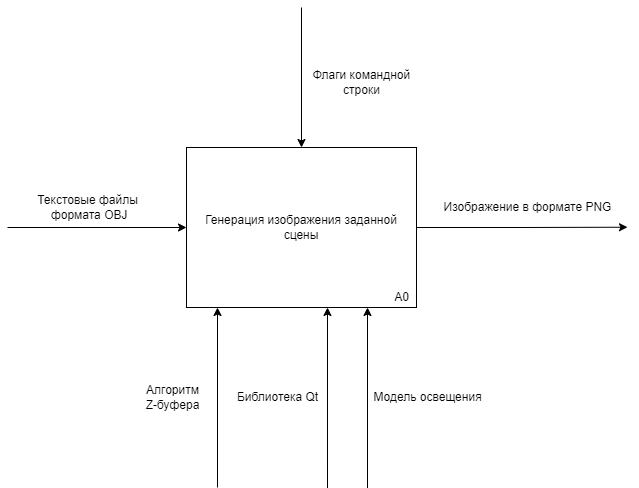
\includegraphics[width=0.7\linewidth]{idef_d.png}}
		\caption{IDEF0 диаграмма работы реализованной программы}
		\label{ris:image}
		\end{figure}
		\section{Формат входных и выходных данных и обоснование выбора}
		Для представления входных данных основным форматом был выбран 
формат файлов OBJ, так как:
		\begin{enumerate} 
        			\item Имеет широкую поддержку экспорта и импорта программного 
обеспечения САПР. Любое программное обеспечение САПР будет 
интерпретировать OBJ модель правильно и последовательно
			\item Легко воспринимается пользователями без изучения дополнительных 
языков программирования и доступен для ручного изменения (не в 
бинарном формате)
			\item В отличие от некоторых аналогов (например, STL) позволяет хранить 
текстуры (в отдельном MTL файле)
			\item Согласно статье [7] формат файла OBJ, благодаря своей нейтральности, является одним из самых популярных форматов обмена для 3D-графики. Он также набирает обороты в индустрии 3D-печати, поскольку отрасль движется к полноцветной печати.
    		\end{enumerate} 
		Для выходных данных был выбран формат файла PNG, так как:
		\begin{enumerate} 
        			\item Качество изображения формата PNG не меняется при любой степени 
сжатия.
			\item Формат является платформонезависимым (в отличие от BMP
файлов, удовлетворяющих только Windows).
			\item Данный формат поддерживает максимальное возможное количество 
цветов.
			\item Является совместимым с утилитой ffmpeg, используемой для 
создания видеофрагмента [6].
			\item Согласно статье [8], среднеквадратическая ошибка (среднее 
различие в квадрате между идеальным и фактическим пиксельными 
значениями) для JPEG файлов на больших изображениях гораздо 
больше, чем у PNG файлов (данные в статье представлены для 
изображения размером 1024x1024 пиксела, в работе используется 
размер 1600x900 пикселов)
    		\end{enumerate} 


		\section{Реализуемые алгоритмы}



		\subsection{Алгоритм Z-буфера}
		Данный алгоритм работает в пространстве изображений, используя буфер
кадра для заполнения интенсивности каждого пикселя, здесь вводится
некоторый Z-буфер (буфер глубины каждого пикселя).
\par Значение каждого нового пикселя, который нужно занести в буфер кадра,
сравнивается с глубиной пикселя, занесенного в Z-буфер. Если сравнение
показывает, что новый пиксель расположен ближе к наблюдателю, то новое
значение Z заносится в буфер и корректируется значение интенсивности.
\par Алгоритм, использующий Z-буфер крайне прост в своей реализации по
сравнению с другими анализируемыми алгоритмами, также не тратится время
на сортировку элементов сцены.
\par Но несмотря на его быстродействие увеличиваются затраты по памяти при
использовании данного алгоритма, запоминается информация по каждому
пикселю изображения.
\par Вычислительная сложность данного алгоритма равна 
\begin{math}
O(n\cdot m\cdot k)
\end{math}, где
\begin{math}
n\cdot m
\end{math} –
количество пикселей в буфере кадра, k – количество полигонов.
\subsubsection{Алгоритм}
\begin{enumerate}
	\item  Всем элементам буфера кадра присвоить фоновое значение;
	\item Инициализировать Z-буфер минимальными значениями глубины;
	\item Выполнить растровую развертку каждого многоугольника сцены:
	\begin{enumerate}
		\item   Для каждого пикселя, связанного с многоугольником вычислить его
глубину \begin{math}
z(x, y)
\end{math};
		\item  Сравнить глубину пикселя со значением, хранимым в Z-буфере. Если
\begin{math}
z(x, y)
\end{math} > \begin{math}
z_b(x, y)
\end{math}, то \begin{math}
z_b(x, y)
\end{math} = \begin{math}
z(x, y)
\end{math} и цвет\begin{math}
(x, y)
\end{math} = цветПикселя;
	\end{enumerate}
	\item Отобразить результат;
\end{enumerate} 
\subsubsection{Математическое содержание алгоритма}
При известном уравнении плоскости, несущей конкретный многоугольник,
вычисление глубины каждого пикселя могут быть произведены пошаговым
способом.
\par При известном уравнении плоскости, несущей конкретный многоугольник,
вычисление глубины каждого пикселя могут быть произведены пошаговым
способом.
\par Уравнение плоскости имеет следующий вид (выражено через z):
\begin{center}
	\begin{math}
		z = \frac{
		ax + by + d
  		}{
  		c
		}
 		\neq 0
	\end{math}
\end{center}
\par Для сканирующей строки \begin{math} y = const\end{math}, глубина пикселя, у которого \begin{math} x_1 = x + \bigtriangleup x\end{math}, поэтому равна:
\begin{center}
	\begin{math}
		z_1 - z = - \frac{
		ax_1 +d
  		}{
  		c
		}
 		+  \frac{
		ax +d
  		}{
  		c
		} = 
 		\frac{
		a(x - x_1)
  		}{
  		c
		}
	\end{math}
\end{center}
\par Отсюда получаем, что
\begin{center}
	\begin{math}
		z_1 = z - \frac{
		a
  		}{
  		c
		}\bigtriangleup x
	\end{math}, 
	\begin{math}
		\bigtriangleup x = 1
	\end{math}, поэтому 
	\begin{math}
		z_1 = z - \frac{
		a
  		}{
  		c
		}
	\end{math}
\end{center}
\par Поскольку в данной задаче для визуализации используется только один вид
многоугольников, а именно треугольник, то нахождение абсцисс точек
пересечения горизонтали со сторонами треугольника будет выглядеть
следующим образом:
\begin{itemize}
	\item Для каждой из сторон треугольника будут записываться параметрические
уравнения вида:
	\begin{center}
	\begin{math}
		x = x_H + (x_K - x_H)t
	\end{math}\\
	\begin{math}
		y = y_H + (y_K - y_H)t
	\end{math}
	\end{center}
	\item После этого для каждой стороны находится параметр \begin{math} t \end{math}при пересечении с горизонталью \begin{math} y = c\end{math}:
	\begin{center}
	\begin{math}
		c = y_H + (y_K - y_H)t
	\end{math}, где 
	\begin{math}
		t = \frac{
		c - y_H
  		}{
  		y_K
		} - y_H
	\end{math}
	\end{center}
	\item Если \begin{math} t \in (0, 1)\end{math} , то рассчитывается абсцисса точки
пересечения горизонтали со стороной треугольника:
	\begin{center} 
	\begin{math}
		x = x_H + (x_K - x_H) \frac{
		c - y_H
  		}{
  		y_K - y_H
		}
	\end{math}
	\end{center}
	\begin{figure}[H]
		\center{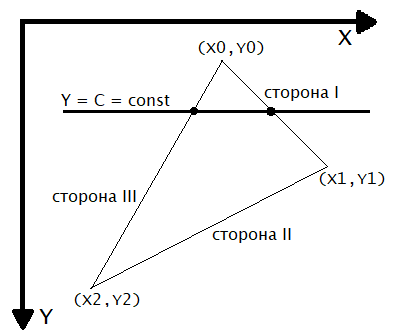
\includegraphics[width=0.49\linewidth]{z_alg.png}}
		\caption{Поиск абсцисс точек пересечения}
		\label{ris:image}
		\end{figure}
\end{itemize}



\subsection{Модифицированный алгоритм Z-буфера}
\begin{enumerate}
\item Для каждого направленного источника света:
	\begin{enumerate}
	\item Инициализировать теневой z-буфер минимальным значением глубины;
	\item Определить теневой z-буфер для источника;
	\end{enumerate}
\item Выполнить алгоритм z-буфера для точки наблюдения. При этом, если
некоторая поверхность оказалась видимой относительно текущей точки
наблюдения, то проверить, видима ли данная точка со стороны источников
света. Для каждого источника света:
	\begin{enumerate}
	\item Координаты рассматриваемой точки \begin{math} (x, y, z) \end{math} линейно преобразовать из вида наблюдателя в координаты \begin{math} (x’, y’, z’) \end{math} на виде из рассматриваемого источника света;
	\item Сравнить значение \begin{math} z_t(x’, y’) \end{math} со значением \begin{math} z’(x’, y’) \end{math}: Если \begin{math} z’(x’, y’) < z_t(x’, y’)\end{math}, то пиксел высвечивается с учётом
его затемнения, иначе точка высвечивается без затемнения;
	\end{enumerate}
\end{enumerate} 




		\subsection{Освещение}
 В данном проекте планеты не будут иметь
свойств зеркального отражения, а, значит, в данном случае уместно только
диффузное отражение, которое описывается по закону Ламберта:
интенсивность отраженного света пропорциональна косинусу угла между
направлением на точечный источник света и нормалью к поверхности.
		\begin{figure}[H]
		\center{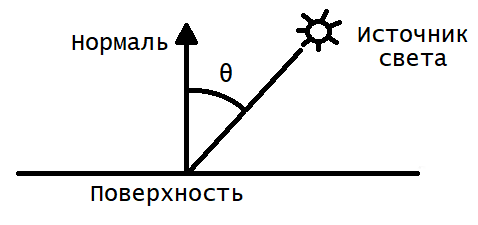
\includegraphics[width=0.49\linewidth]{light.png}}
		\caption{Матовая поверхность}
		\label{ris:image}
		\end{figure}
		\begin{center}
		\begin{math}
		I = I_i \cdot K \cdot \cos (\theta)
		\end{math}
		, где К -- коэффициент свойства материалла поверхности,
		\begin{math}
		I_i
		\end{math}
		-- интенсивность источника света
		\end{center}

		Для определения цвета матовой поверхности определяется комбинацией
собственного цвета поверхности и цвета излучения источника света. Также, как
можно заметить, в формуле имеется косинус угла вектора источника света в
пространстве между вектором нормали к самой поверхности, данную, величину
можно определить при помощи скалярного произведения.
		\par Пусть есть две точки --
		\begin{math}
		A(x_A, y_A, z_A)
		\end{math}
		, принадлежащая поверхности, и точка
		\begin{math}
		B(x_B, y_B, z_B)
		\end{math}
		, задающая положение источника в пространстве, также имеется
		вектор нормали
		\begin{math}
		N(x_N, y_N, z_N)
		\end{math}
		, тогда вектор от точки поверхности к источнику
		света имеет следующие координаты:
		\begin{center}
		\begin{math}
		V(x_B - x_A, y_B - y_A, z_B - z_A)
		\end{math}
		\end{center}
		Отсюда следует, что:
		\begin{center}
		\begin{math}
		N \cdot V =\mid N\mid \cdot \mid V \mid\cdot \cos (\theta)
		\end{math}
		\end{center}
		После преобразований и подстановок получается следующее:
		\begin{center}
		\begin{math}
		N \cdot V = x_N x_V + y_N y_V + z_N z_V
		\end{math}
		\end{center}
		Следовательно с учетом того, что в программе будут использоваться
единичные вектора нормали (уменьшает количество вычислений), получаем
следующее:
		\begin{center}
		\begin{math}
		\cos (\theta) = \frac{
		x_N(x_B - x_A)+y_N(y_B-y_A)+z_N(z_B-z_A)
  		}{
  		\sqrt{(x_B - x_A)^2 + (y_B - y_A)^2 + (z_B - z_A)^2}
		} = \frac{
		x_N(x_B - x_A)+y_N(y_B-y_A)+z_N(z_B-z_A)
  		}{
  		\mid V \mid
		}
		\end{math}
		\end{center}


		\subsection{Метод закраски Гуро}
		Поскольку данный метод основан на билинейной интерполяции вектора
нормали. Определение интерполированных значений удобно выполнять на
моменте заполнения полигона, например, совместить с алгоритмом
визуализации изображения. После этого рассматривается заполнение грани
горизонталями в экранных координатах.
		\par Рассмотрим основные этапы данного алгоритма:
		\begin{enumerate}
\item Вычисление векторов нормалей к каждой грани;
\item Вычисление векторов нормалей к каждой вершине грани через
усреднение нормалей к граням;
\item Вычисление интенсивностей в вершинах граней;
\item Интерполяция интенсивности вдоль ребер грани;
\item Линейная интерполяция вдоль сканирующей строки;
	\begin{figure}[H]
		\center{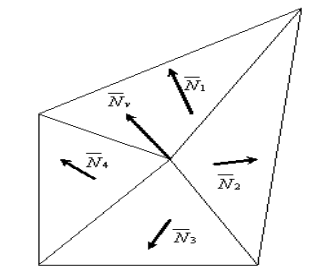
\includegraphics[width=0.49\linewidth]{interpol.png}}
		\caption{Усреднение нормалей к граням}
		\label{ris:image}
	\end{figure}
\end{enumerate}
\par Интерполированная интенсивность \begin{math}I\end{math} в точке \begin{math}(x, y) \end{math} определяется из пропорции:
\begin{center}
		\begin{math}
		\frac{
		I - I_1
  		}{
  		x - x_1
		} = \frac{
		I_2 - I_1
  		}{
  		x_2 - x_1
		}
		\end{math}, выражая отсюда 
		\begin{math}
		I
		\end{math}, получаем:
		\begin{math}
		I = I_1 + \frac{
		(I_2 - I_1) \cdot (x - x_1)
  		}{
  		(x_2 - x_1)
		} 
		\end{math}
\end{center}
	\begin{figure}[H]
		\center{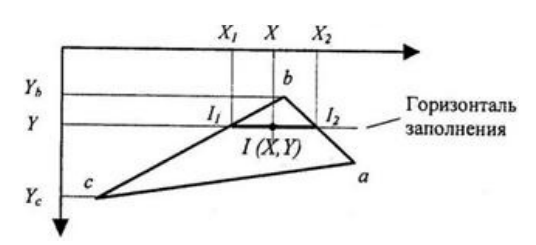
\includegraphics[width=0.49\linewidth]{interpol_2.png}}
		\caption{Интерполяция значений интенсивности}
		\label{ris:image}
	\end{figure}
Значения \begin{math}I_1\end{math} и \begin{math}I_2\end{math} на концах горизонтального отрезка является интерполяцией
интенсивности в вершинах:
\begin{center}
		\begin{math}
		\frac{
		l_1 - l_b
  		}{
  		Y - Y_b
		} = \frac{
		l_c - l_b
  		}{
  		Y_c - Y_b
		}
		\end{math}, а также 
		\begin{math}
		\frac{
		l_2 - l_b
  		}{
  		Y - Y_b
		} = \frac{
		l_a - l_b
  		}{
  		Y_a - Y_b
		}
		\end{math}, откуда получается, что 
		\begin{math}
		l_1 = l_b + \frac{
		(l_c - l_b)(Y - Y_b)
  		}{
  		Y_c - Y_b
		} 
		\end{math} и
		\begin{math}
		l_2 = l_b + \frac{
		(l_a - l_b)(Y - Y_b)
  		}{
  		Y_a - Y_b
		} 
		\end{math}
\end{center}

	\section{Сценарий Gitlab CI/CD}
	На рисунке 2.5 продемонстрированы зависимости сценария CI/CD.
	\begin{figure}[H]
		\center{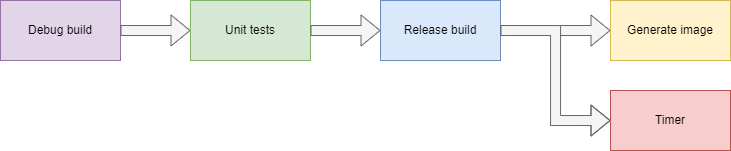
\includegraphics[width=1\linewidth]{CIDiagram.png}}
		\caption{диаграмма зависимостей в сценарии Gitlab CI/CD}
		\label{ris:image}
	\end{figure}
\par Сценарий состоит из 5 стадий:
\begin{itemize}
\item build\_debug — отладочная сборка программы
В этой стадии одно задание — Debug build, в котором производится 
сборка отладочной версии программы.
\item test — модульное тестирование программы
В этой стадии одно задание — Unit tests, в котором осуществляется 
модульное тестирование функции SetAutoNormal() из заголовочного файла 
surface.h.
\item build\_release — сборка выпускаемой версии программы
В этой стадии одно задание — Release build, в котором производится 
сборка версии программы для выпуска.
\item gen\_image --  генерация изображения заданной сцены
\item calculate\_time -- проведение замерного эксперимента и построение графиков
\end{itemize}
\par Описание зависимостей сценария CI/CD:
\begin{itemize}
\item Задание сборки отладочной версии программы не имеет 
зависимостей, так как отладочная сборка первична.
\item Задание модульного тестирования программного модуля зависит от 
задания сборки отладочной версии программы, так как для запуска 
тестов необходимо наличие исполняемого файла программы, 
который может быть получен в результате отладочной сборки.
\item Задание выпускаемой сборки программы зависит от задания 
модульного тестирования программы (соответственно, и от задания 
сборки отладочной версии программы, явно указывать косвенную 
зависимость в сценарии CI/CD не нужно), так как выпускаемая 
версия программы не должна содержать в себе ошибок.
\item Задание проведения замерного эксперимента зависит от задания 
выпускаемой сборки, так как для исследования времени работы 
программы необходим исполняемый файл программы, для которого 
обеспечена защита от возникновения ошибочных ситуаций и 
оптимизация работы программы.
\item Задания генерации изображения заданной сцены зависит от задания 
выпускаемой сборки, так как для генерации изображений сцены необходим исполняемый файл программы, для которого обеспечена 
защита от возникновения ошибочных ситуаций и оптимизация 
работы программы.
\end{itemize}
\par Далее приведено содержание файла .gitlab-ci.yml со сценарием CI/CD
\begin{lstlisting}[label=some-code,caption= содержание файла .gitlab-ci.yml со сценарием CI/CD]
image: rabits/qt:5.15-desktop

stages: 
 	- build_debug
  	- test
  	- build_release
  	- gen_image
  	- calculate_time

Debug build:

 	 stage: build_debug

  	script:
    		- cd new_code
    		- qmake CONFIG+=debug new_code.pro 
    		- make

	artifacts:
		paths:
      			- new_code/new_code
    		expire_in: 1 day

Unit tests:

  	stage: test

  	script:
    		- cd new_code
    		- ./new_code -test
  	needs:
    		- job: Debug build
      	artifacts: true

Release build:

 	 stage: build_release

  	script:
    		- cd new_code
    		- qmake CONFIG+=release new_code.pro
    		- make

  	artifacts:
    		paths:
      			- new_code/new_code
    		expire_in: 1 day
  	needs:
    		- Unit tests
  	when: manual


Generate image:

  	stage: gen_image

  	script:
    		- cd new_code
    		- bash gen_image.sh
  	artifacts:
   		 paths:
      			- new_code/img.png
    		expire_in: 7 days
  	needs:
    		- job: Release build
      		artifacts: true

Timer:

  	stage: calculate_time
	image: python
  	before_script:
    		- pip install matplotlib
  	script:
    		- cd new_code
    		- bash gen_time.sh
  	artifacts:
    		paths:
      			- new_code/graph.png
    		expire_in: 7 days
  	needs:
    		- job: Release build
      		artifacts: true
\end{lstlisting}
\section{Docker}
В сценарии Gitlab CI/CD были использованы образы docker с Docker Hub, 
удовлетворяющие задачам соответствующих заданий конвейера. Ниже 
приведено описание данных образов и обоснование их использования:
\begin{enumerate} 
\item rabits/qt:5.15-desktop
Образ rabits/qt:5.15-desktop представляет собой набор пакетов для 
сборки и исполнения программ в фреймворке Qt. Он использовался 
для всех заданий, кроме Timer, так как этому 
заданию требовалось иное специфичное окружение, а остальным 
была необходима сборка и исполнение программы, следовательно, 
библиотеки Qt. Зависимости образа:
\begin{itemize}
\item unzip
\item git
\item openssh-client
\item ca-certificates
\item locales
\item sudo
\item curl
\item make
\item openjdk-8-jdk-headless
\item openjdk-8-jre-headless
\item ant
\item libsm6
\item libice6
\item libxext6
\item libxrender1
\item libxkbcommon-x11-0
\item libfontconfig
\item libdbus-1-3
\item libx11-xcb1
\item libc6:i386
\item libncurses5:i386
\item libstdc++6:i386
\item libz1:i386
\end{itemize}
\item python
Образ python с необходимыми для запуска программ на языке Python
пакетами был использован в задании Timer, так как в ходе этого 
задания было необходимо запустить скрипт для построения графика 
по полученным временным характеристикам с помощью библиотеки 
matplotlib языка Python. Зависимости образа:
\begin{itemize}
\item gnupg
\item dirmngr
\item git 
\item mercurial 
\item openssh-client 
\item subversion 
\item procps
\item autoconf 
\item automake 
\item bzip2 
\item dpkg-dev 
\item file 
\item g++ 
\item gcc 
\item imagemagick 
\item libbz2-dev 
\item libc6-dev 
\item libcurl4-openssl-dev 
\item libdb-dev 
\item libevent-dev 
\item libffi-dev 
\item libgdbm-dev 
\item libglib2.0-dev 
\item libgmp-dev 
\item libjpeg-dev 
\item libkrb5-dev 
\item liblzma-dev 
\item libmagickcore-dev 
\item libmagickwand-dev 
\item libmaxminddb-dev 
\item libncurses5-dev 
\item libncursesw5-dev 
\item libpng-dev 
\item libpq-dev 
\item libreadline-dev 
\item libsqlite3-dev 
\item libssl-dev 
\item libtool 
\item libwebp-dev 
\item libxml2-dev 
\item libxslt-dev 
\item libyaml-dev
\item make 
\item patch 
\item unzip 
\item xz-utils 
\item zlib1g-dev
\end{itemize}

\end{enumerate} 
\section{Модульное тестирование}
Было произведено тестирование одного из модулей программы с помощью 
библиотеки testlib и фреймворка Qt Test.
\par Для тестирования был выбран модуль Surface, из которого была выбрана 
функция SetAutoNormal для примера теста, как наиболее простая для понимания и подбора 
данных для тестирования. Создан класс Test, наследуемый от класса 
QObject. В публичном слоте находится конструктор класса, а в приватном —
непосредственно создаваемые тесты.
\begin{lstlisting}[label=some-code,caption= Класс Test для тестирования модуля Surface]
class Test : public QObject {
    Q_OBJECT
public:
    explicit Test(QObject* parent = nullptr);

private slots:
    void test_01();
};
\end{lstlisting}
\par Таким образом, чтобы добавить новый тест, достаточно создать новый 
приватный слот. В данном случае добавление теста будет выглядеть следующим 
образом:
\begin{lstlisting}[label=some-code,caption= пример добавления нового модульного теста]
private slots:
    void test_01();
    void test_02();
\end{lstlisting}
\par Ниже приведен листинг реализации конкретного теста проверки рассчета нормали к заданной поверхности. Проверка корректности полученного результата производится с помощью макросов фреймворка Qt Test. В данном примере используется макрос 
QCOMPARE, сравнивающий ожидаемое значение с полученным.
\begin{lstlisting}[label=some-code,caption= реализация модульного теста test\_01]
void Test::test_01()
{
    QColor cl(255, 4, 33);
    QRgb r = cl.rgb();

    QVector3D p1(0.0, 10.0, 0.0);
    QVector3D p2(0.0, 0.0, 0.0);
    QVector3D p3(0.0, 0.0, 10.0);

    Surface c(Polygon(p1 , p2 , p3 , r));

    c.SetAutoNormal();
    QVector3D n = c.GetNormal().getNorm();

    QCOMPARE(qFuzzyCompare(n.x(), -100.0), true);
    QCOMPARE(qFuzzyCompare(n.y(), 0.0), true);
    QCOMPARE(qFuzzyCompare(n.z(), 0.0), true);
}
\end{lstlisting}
\par Функция qFuzzyCompare используется для корректного сравнения чисел с 
плавающей точкой, так как QCOMPARE сравнивает числа с помощью оператора 
«==». Такое сравнение не используется для чисел с плавающей точкой, но 
подходит для сравнения значений типа bool, что и показано в приведенном 
примере.
\section{Реализация управления из командной строки}
Для автоматизации работы программы и использования сценария было 
необходимо реализовать передачу в программу аргументов командной строки и 
их распознавание самой программой. Для этого была использована библиотека 
getopt [12], позволяющая выполнить «сканирование» аргументов командной 
строки и их обработку. Конкретно была использована одноименная функция 
getopt, которая последовательно перебирает переданные параметры в программу 
в соответствии с заданной строкой параметров, содержащей имена параметров и 
признак наличия передаваемого значения («:»).
Перечень используемых параметров:
\begin{itemize}
\item Флаг «-f» — указание программе о том, что нужно отрисовать первую сцену и сохранить полученное изображение.
\item Флаг «-s» — указание программе о том, что нужно отрисовать вторую сцену и сохранить полученное изображение.
\item Флаг «-t» — указание программе о том, что нужно отрисовать третью сцену и сохранить полученное изображение.
\item Флаг «-time» — указание программе о том, что нужно провести замер времени и вызвать python скрипт, который сгенерирует графики.
\item Флаг «-test» — указание программе о том, что проводится модульное тестирование.
\end{itemize}
\begin{lstlisting}[label=some-code,caption= пример вызова программы для замеров времени ]
#!/bin/bash

./new_code -timer 
\end{lstlisting}
\section{Пример работы программы}
На рисунках 2.7–2.9 представлены изображения, полученные в результате 
работы программы с тремя разными сценами, содержащими модели с 
различным количеством полигонов.

\begin{figure}[H]
		\center{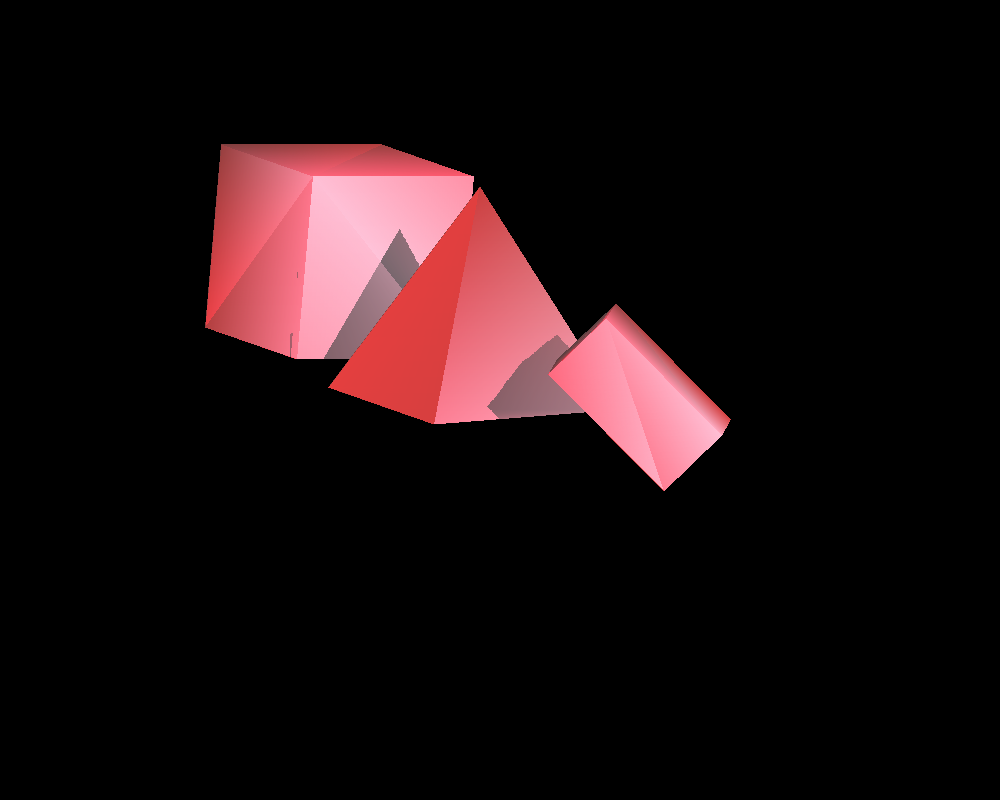
\includegraphics[width=0.8\linewidth]{scene_1.png}}
		\caption{пример №1 работы программы}
		\label{ris:image}
	\end{figure}
\begin{figure}[H]
		\center{
\includegraphics[width=0.8\linewidth]{scene_2.png}}
		\caption{пример №2 работы программы}
		\label{ris:image}
	\end{figure}
\begin{figure}[H]
		\center{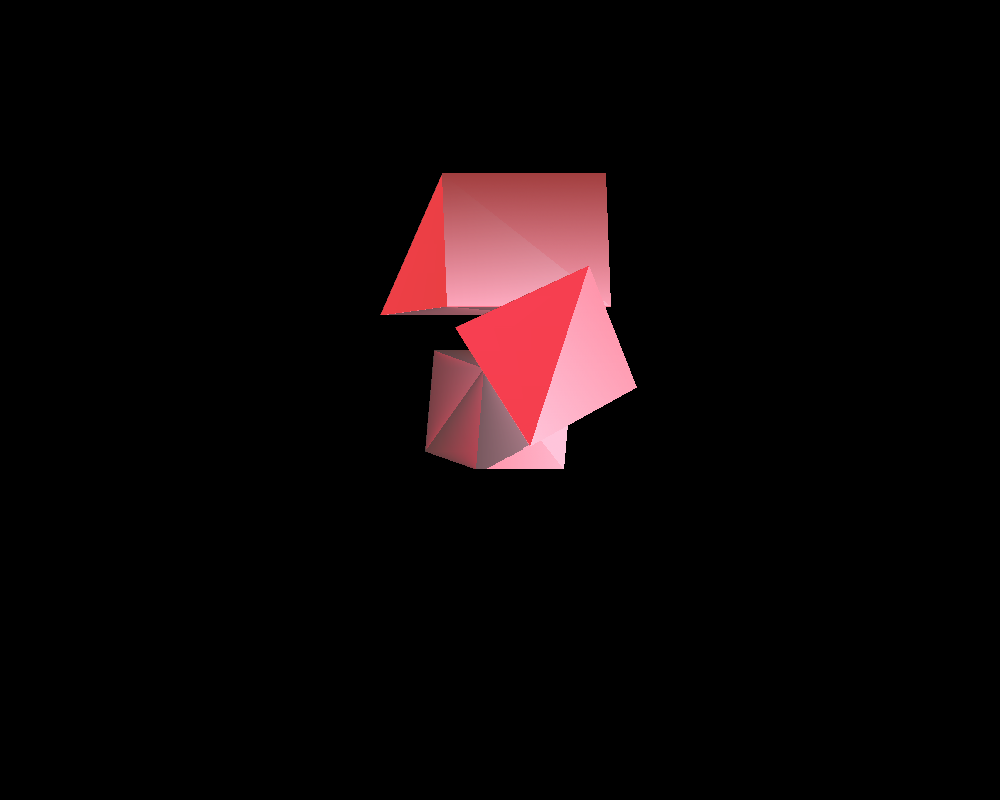
\includegraphics[width=0.8\linewidth]{scene_3.png}}
		\caption{пример №3 работы программы}
		\label{ris:image}
	\end{figure}

\chapter*{Заключение}
\addcontentsline{toc}{chapter}{Заключение}
Во время выполнения поставленной задачи была изучена документация Qt, Qt Test, Qt Widgets, Gitlab CI/CD, Docker, ffmpeg. Были рассмотрены и
реализованы алгоритмы удаления невидимых линий,
построения теней, методы закрашивания и модели освещенности. Был создан сценарий автоматизации сборки, тестирования и 
получения данных будущего исследования. Было создано три сцены и проведено 
модульное тестирование для демонстрации работоспособности конвейера.
Также был реализован замерный эксперимент зависимости времени выполнения 
программы от числа полигонов.
\par В ходе выполнения технологической практики были выполнены все 
поставленные цели и задачи.
\par Данная работа помогла закрепить полученные навыки в области 
компьютерной графики, приобрести опыт самостоятельной разработки 
программного продукта и проектирования программного обеспечения и изучить 
средства автоматизации развёртывания, сборки и тестирования программы.

		\chapter*{Список литературы}
\addcontentsline{toc}{chapter}{Список литературы}
		\begin{enumerate} 
        			\item Документация по Gitlab CI/CD (Электронный ресурс). \\Режим 
доступа: https://docs.gitlab.com/ee/ci (дата обращения: 16.07.2022).
			\item Документация по Docker (Электронный ресурс).\\Режим доступа: 
https://docs.docker.com (дата обращения: 16.07.2022).
			\item Документация библиотеки Qt (Электронный ресурс).\\ Режим доступа: 
https://doc.qt.io (дата обращения: 01.07.2022). 
			\item Документация библиотеки Qt Widgets (Электронный ресурс). \\Режим 
доступа: https://doc.qt.io/qt-6/qtwidgets-index.html (дата обращения: 
01.07.2022).
			\item Документация библиотеки Qt Test (Электронный ресурс). \\Режим 
доступа: https://doc.qt.io/qt-6/qttest-index.html (дата обращения: 
15.07.2022).
			\item Документация по ffmpeg (Электронный ресурс). \\Режим доступа: 
https://ffmpeg.org/documentation.html (дата обращения: 18.07.2022).
			\item The Most Common 3D File Formats in 2022 (Электронный ресурс) \\ Режим доступа: https://all3dp.com/2/most-common-3d-file-formats-model/ (дата обращения: 18.07.2022)
			\item Comparison of different image formats using LSB Steganography 
(Электронный ресурс). \\Режим доступа: 
https://ieeexplore.ieee.org/stamp/stamp.jsp?tp=\&arnumber=8269657 
(дата обращения 15.07.2022)
			\item Д. Роджерс. Алгоритмические основы машинной графики./Д.
Роджерс. – М.: Мир, 1989. – 512с
			\item Peter Shirley and Steve Marschner. Fundamentals of Computer
Graphics - 3rd Edition, 2009. 782с.
			\item Куров А.В., Курс лекций по дисциплине «Компьютерная графика»
			\item Документация по библиотеке getopt. (Электронный ресурс). \\Режим 
доступа: https://ru.manpages.org/getopt/3 (дата обращения: 
05.07.2022)

    		\end{enumerate} 
\end{document}